\chapter{\dune{} ND Event Pile-up Study Data}
\label{chap:pile-up-data}

\section{\SI{2}{\mega\watt} Beam at \SI{80}{\giga\electronvolt} Proton Energy}

\begin{figure}[htb]
	\centering
	\includegraphics[width=\textwidth]{pile-up/2MW/abs_2d_missed}
	\caption{2D histogram of missed energy versus true photon energy for a simple \Pgpz-induced EM shower reconstruction algorithm based on a cone-cylinder union.
		All energy deposited outside of the cone-cylinder union is counted as missed.
		The simulated beam intensity is \SI{2}{\mega\watt} at \SI{80}{\giga\electronvolt} proton energy.
		Under the number of entries, a detailed list of the number of entries inside (centre) and outside (edges and corners) the depicted area of the histogram is given (under- and overflow).}
\end{figure}

\begin{figure}[htb]
	\centering
	\includegraphics[width=\textwidth]{pile-up/2MW/missed_abs_x}
	\caption{Missed energy versus true photon energy for a simple \Pgpz-induced EM shower reconstruction algorithm based on a cone-cylinder union.
		All energy deposited outside of the cone-cylinder union is counted as missed.
		The simulated beam intensity is \SI{2}{\mega\watt} at \SI{80}{\giga\electronvolt} proton energy.}
\end{figure}

\begin{figure}[htb]
	\centering
	\includegraphics[width=\textwidth]{pile-up/2MW/rel_2d_missed}
	\caption{2D histogram of missed energy fraction versus true photon energy for a simple \Pgpz-induced EM shower reconstruction algorithm based on a cone-cylinder union.
		All energy deposited outside of the cone-cylinder union is counted as missed.
		The simulated beam intensity is \SI{2}{\mega\watt} at \SI{80}{\giga\electronvolt} proton energy.
		Under the number of entries, a detailed list of the number of entries inside (centre) and outside (edges and corners) the depicted area of the histogram is given (under- and overflow).}
\end{figure}

\begin{figure}[htb]
	\centering
	\includegraphics[width=\textwidth]{pile-up/2MW/missed_rel_x}
	\caption{Missed energy fraction versus true photon energy for a simple \Pgpz-induced EM shower reconstruction algorithm based on a cone-cylinder union.
		All energy deposited outside of the cone-cylinder union is counted as missed.
		The simulated beam intensity is \SI{2}{\mega\watt} at \SI{80}{\giga\electronvolt} proton energy.}
\end{figure}

\begin{figure}[htb]
	\centering
	\includegraphics[width=\textwidth]{pile-up/2MW/missed_rel_y}
	\caption{Cumulatetive fraction of photons versus missed energy fraction for a simple \Pgpz-induced EM shower reconstruction algorithm based on a cone-cylinder union.
		All energy deposited outside of the cone-cylinder union is counted as missed.
		The curve depicts the fraction of photons on the y-axis with a missed energy fraction equal to or lower than the corresponding value on the x-axis.
		The simulated beam intensity is \SI{2}{\mega\watt} at \SI{80}{\giga\electronvolt} proton energy.}
\end{figure}

\begin{figure}[htb]
	\centering
	\includegraphics[width=\textwidth]{pile-up/2MW/abs_2d_other}
	\caption{2D histogram of misidentified energy versus true neutrino energy for a simple \Pgpz-induced EM shower reconstruction algorithm based on a cone-cylinder union.
		All energy deposited inside the cone-cylinder union by descendants of parent neutrinos different from the parent of the corresponding \Pgpz photon is counted as misidentified.
		The simulated beam intensity is \SI{2}{\mega\watt} at \SI{80}{\giga\electronvolt} proton energy.
		Under the number of entries, a detailed list of the number of entries inside (centre) and outside (edges and corners) the depicted area of the histogram is given (under- and overflow).}
\end{figure}

\begin{figure}[htb]
	\centering
	\includegraphics[width=\textwidth]{pile-up/2MW/abs_2d_notmu}
	\caption{2D histogram of misidentified energy versus true neutrino energy for a simple \Pgpz-induced EM shower reconstruction algorithm based on a cone-cylinder union.
		Energy deposited inside the cone-cylinder union by descendants of parent neutrinos different from the parent of the corresponding \Pgpz photon is counted as misidentified.
		Any energy deposited by muons is excluded.
		The simulated beam intensity is \SI{2}{\mega\watt} at \SI{80}{\giga\electronvolt} proton energy.
		Under the number of entries, a detailed list of the number of entries inside (centre) and outside (edges and corners) the depicted area of the histogram is given (under- and overflow).}
\end{figure}

\begin{figure}[htb]
	\centering
	\includegraphics[width=\textwidth]{pile-up/2MW/abs_2d_neutral}
	\caption{2D histogram of misidentified energy versus true neutrino energy for a simple \Pgpz-induced EM shower reconstruction algorithm based on a cone-cylinder union.
		Energy deposited inside the cone-cylinder union by descendants of parent neutrinos different from the parent of the corresponding \Pgpz photon is counted as misidentified.
		Only energy deposited by photons, neutrons, or any of their descendants is included.
		The simulated beam intensity is \SI{2}{\mega\watt} at \SI{80}{\giga\electronvolt} proton energy.
		Under the number of entries, a detailed list of the number of entries inside (centre) and outside (edges and corners) the depicted area of the histogram is given (under- and overflow).}
\end{figure}

\begin{figure}[htb]
	\centering
	\includegraphics[width=\textwidth]{pile-up/2MW/misid_abs_x}
	\caption{Misidentified energy versus true neutrino energy for a simple \Pgpz-induced EM shower reconstruction algorithm based on a cone-cylinder union.
		All energy deposited inside the cone-cylinder union by descendants of parent neutrinos different from the parent of the corresponding \Pgpz photon is counted as misidentified.
		Colour indicates different selections of misidentified energy: total (cyan); excluding depositions from muons (red); deposition from photons, neutrons, and their descendants only (blue).
		The simulated beam intensity is \SI{2}{\mega\watt} at \SI{80}{\giga\electronvolt} proton energy.}
\end{figure}

\begin{figure}[htb]
	\centering
	\includegraphics[width=\textwidth]{pile-up/2MW/rel_2d_other}
	\caption{2D histogram of misidentified energy fraction versus true neutrino energy for a simple \Pgpz-induced EM shower reconstruction algorithm based on a cone-cylinder union.
		All energy deposited inside the cone-cylinder union by descendants of parent neutrinos different from the parent of the corresponding \Pgpz photon is counted as misidentified.
		The simulated beam intensity is \SI{2}{\mega\watt} at \SI{80}{\giga\electronvolt} proton energy.
		Under the number of entries, a detailed list of the number of entries inside (centre) and outside (edges and corners) the depicted area of the histogram is given (under- and overflow).}
\end{figure}

\begin{figure}[htb]
	\centering
	\includegraphics[width=\textwidth]{pile-up/2MW/rel_2d_notmu}
	\caption{2D histogram of misidentified energy fraction versus true neutrino energy for a simple \Pgpz-induced EM shower reconstruction algorithm based on a cone-cylinder union.
		Energy deposited inside the cone-cylinder union by descendants of parent neutrinos different from the parent of the corresponding \Pgpz photon is counted as misidentified.
		Any energy deposited by muons is excluded.
		The simulated beam intensity is \SI{2}{\mega\watt} at \SI{80}{\giga\electronvolt} proton energy.
		Under the number of entries, a detailed list of the number of entries inside (centre) and outside (edges and corners) the depicted area of the histogram is given (under- and overflow).}
\end{figure}

\begin{figure}[htb]
	\centering
	\includegraphics[width=\textwidth]{pile-up/2MW/rel_2d_neutral}
	\caption{2D histogram of misidentified energy fraction versus true neutrino energy for a simple \Pgpz-induced EM shower reconstruction algorithm based on a cone-cylinder union.
		Energy deposited inside the cone-cylinder union by descendants of parent neutrinos different from the parent of the corresponding \Pgpz photon is counted as misidentified.
		Only energy deposited by photons, neutrons, or any of their descendants is included.
		The simulated beam intensity is \SI{2}{\mega\watt} at \SI{80}{\giga\electronvolt} proton energy.
		Under the number of entries, a detailed list of the number of entries inside (centre) and outside (edges and corners) the depicted area of the histogram is given (under- and overflow).}
\end{figure}

\begin{figure}[htb]
	\centering
	\includegraphics[width=\textwidth]{pile-up/2MW/misid_rel_x}
	\caption{Misidentified energy fraction versus true neutrino energy for a simple \Pgpz-induced EM shower reconstruction algorithm based on a cone-cylinder union.
		All energy deposited inside the cone-cylinder union by descendants of parent neutrinos different from the parent of the corresponding \Pgpz photon is counted as misidentified.
		Colour indicates different selections of misidentified energy: total (cyan); excluding depositions from muons (red); deposition from photons, neutrons, and their descendants only (blue).
		The simulated beam intensity is \SI{2}{\mega\watt} at \SI{80}{\giga\electronvolt} proton energy.}
\end{figure}

\begin{figure}[htb]
	\centering
	\includegraphics[width=\textwidth]{pile-up/2MW/misid_rel_y}
	\caption{Cumulative fraction of neutrinos versus misidentified energy fraction for a simple \Pgpz-induced EM shower reconstruction algorithm based on a cone-cylinder union.
		All energy deposited inside the cone-cylinder union by descendants of parent neutrinos different from the parent of the corresponding \Pgpz photon is counted as misidentified.
		Colour indicates different selections of misidentified energy: total (cyan); excluding depositions from muons (red); deposition from photons, neutrons, and their descendants only (blue).
		The curve depicts the fraction of neutrinos on the y-axis with a misidentified energy fraction equal to or lower than the corresponding value on the x-axis.
		The simulated beam intensity is \SI{2}{\mega\watt} at \SI{80}{\giga\electronvolt} proton energy.}
\end{figure}

\clearpage


\section{\SI{2}{\mega\watt} Beam at \SI{80}{\giga\electronvolt} Proton Energy, XZ Projection}

\begin{figure}[htb]
	\centering
	\includegraphics[width=\textwidth]{pile-up/2MW_XZ/abs_2d_missed}
	\caption{2D histogram of missed energy versus true photon energy for a simple \Pgpz-induced EM shower reconstruction algorithm based on a cone-cylinder union.
		All energy deposited outside of the cone-cylinder union is counted as missed.
		The simulated beam intensity is \SI{2}{\mega\watt} at \SI{80}{\giga\electronvolt} proton energy.
		As a primitive simulation of a wire readout, only X and Z coordinates are used for the energy reconstruction.
		Under the number of entries, a detailed list of the number of entries inside (centre) and outside (edges and corners) the depicted area of the histogram is given (under- and overflow).}
\end{figure}

\begin{figure}[htb]
	\centering
	\includegraphics[width=\textwidth]{pile-up/2MW_XZ/missed_abs_x}
	\caption{Missed energy versus true photon energy for a simple \Pgpz-induced EM shower reconstruction algorithm based on a cone-cylinder union.
		All energy deposited outside of the cone-cylinder union is counted as missed.
		The simulated beam intensity is \SI{2}{\mega\watt} at \SI{80}{\giga\electronvolt} proton energy.
		As a primitive simulation of a wire readout, only X and Z coordinates are used for the energy reconstruction.
		Under the number of entries, a detailed list of the number of entries inside (centre) and outside (edges and corners) the depicted area of the histogram is given (under- and overflow).}
\end{figure}

\begin{figure}[htb]
	\centering
	\includegraphics[width=\textwidth]{pile-up/2MW_XZ/rel_2d_missed}
	\caption{2D histogram of missed energy fraction versus true photon energy for a simple \Pgpz-induced EM shower reconstruction algorithm based on a cone-cylinder union.
		All energy deposited outside of the cone-cylinder union is counted as missed.
		The simulated beam intensity is \SI{2}{\mega\watt} at \SI{80}{\giga\electronvolt} proton energy.
		As a primitive simulation of a wire readout, only X and Z coordinates are used for the energy reconstruction.
		Under the number of entries, a detailed list of the number of entries inside (centre) and outside (edges and corners) the depicted area of the histogram is given (under- and overflow).}
\end{figure}

\begin{figure}[htb]
	\centering
	\includegraphics[width=\textwidth]{pile-up/2MW_XZ/missed_rel_x}
	\caption{Missed energy fraction versus true photon energy for a simple \Pgpz-induced EM shower reconstruction algorithm based on a cone-cylinder union.
		All energy deposited outside of the cone-cylinder union is counted as missed.
		The simulated beam intensity is \SI{2}{\mega\watt} at \SI{80}{\giga\electronvolt} proton energy.
		As a primitive simulation of a wire readout, only X and Z coordinates are used for the energy reconstruction.}
\end{figure}

\begin{figure}[htb]
	\centering
	\includegraphics[width=\textwidth]{pile-up/2MW_XZ/missed_rel_y}
	\caption{Cumulatetive fraction of photons versus missed energy fraction for a simple \Pgpz-induced EM shower reconstruction algorithm based on a cone-cylinder union.
		All energy deposited outside of the cone-cylinder union is counted as missed.
		The curve depicts the fraction of photons on the y-axis with a missed energy fraction equal to or lower than the corresponding value on the x-axis.
		The simulated beam intensity is \SI{2}{\mega\watt} at \SI{80}{\giga\electronvolt} proton energy.
		As a primitive simulation of a wire readout, only X and Z coordinates are used for the energy reconstruction.}
\end{figure}

\begin{figure}[htb]
	\centering
	\includegraphics[width=\textwidth]{pile-up/2MW_XZ/abs_2d_other}
	\caption{2D histogram of misidentified energy versus true neutrino energy for a simple \Pgpz-induced EM shower reconstruction algorithm based on a cone-cylinder union.
		All energy deposited inside the cone-cylinder union by descendants of parent neutrinos different from the parent of the corresponding \Pgpz photon is counted as misidentified.
		The simulated beam intensity is \SI{2}{\mega\watt} at \SI{80}{\giga\electronvolt} proton energy.
		As a primitive simulation of a wire readout, only X and Z coordinates are used for the energy reconstruction.
		Under the number of entries, a detailed list of the number of entries inside (centre) and outside (edges and corners) the depicted area of the histogram is given (under- and overflow).}
\end{figure}

\begin{figure}[htb]
	\centering
	\includegraphics[width=\textwidth]{pile-up/2MW_XZ/abs_2d_notmu}
	\caption{2D histogram of misidentified energy versus true neutrino energy for a simple \Pgpz-induced EM shower reconstruction algorithm based on a cone-cylinder union.
		Energy deposited inside the cone-cylinder union by descendants of parent neutrinos different from the parent of the corresponding \Pgpz photon is counted as misidentified.
		Any energy deposited by muons is excluded.
		The simulated beam intensity is \SI{2}{\mega\watt} at \SI{80}{\giga\electronvolt} proton energy.
		As a primitive simulation of a wire readout, only X and Z coordinates are used for the energy reconstruction.
		Under the number of entries, a detailed list of the number of entries inside (centre) and outside (edges and corners) the depicted area of the histogram is given (under- and overflow).}
\end{figure}

\begin{figure}[htb]
	\centering
	\includegraphics[width=\textwidth]{pile-up/2MW_XZ/abs_2d_neutral}
	\caption{2D histogram of misidentified energy versus true neutrino energy for a simple \Pgpz-induced EM shower reconstruction algorithm based on a cone-cylinder union.
		Energy deposited inside the cone-cylinder union by descendants of parent neutrinos different from the parent of the corresponding \Pgpz photon is counted as misidentified.
		Only energy deposited by photons, neutrons, or any of their descendants is included.
		The simulated beam intensity is \SI{2}{\mega\watt} at \SI{80}{\giga\electronvolt} proton energy.
		As a primitive simulation of a wire readout, only X and Z coordinates are used for the energy reconstruction.
		Under the number of entries, a detailed list of the number of entries inside (centre) and outside (edges and corners) the depicted area of the histogram is given (under- and overflow).}
\end{figure}

\begin{figure}[htb]
	\centering
	\includegraphics[width=\textwidth]{pile-up/2MW_XZ/misid_abs_x}
	\caption{Misidentified energy versus true neutrino energy for a simple \Pgpz-induced EM shower reconstruction algorithm based on a cone-cylinder union.
		All energy deposited inside the cone-cylinder union by descendants of parent neutrinos different from the parent of the corresponding \Pgpz photon is counted as misidentified.
		Colour indicates different selections of misidentified energy: total (cyan); excluding depositions from muons (red); deposition from photons, neutrons, and their descendants only (blue).
		The simulated beam intensity is \SI{2}{\mega\watt} at \SI{80}{\giga\electronvolt} proton energy.
		As a primitive simulation of a wire readout, only X and Z coordinates are used for the energy reconstruction.}
\end{figure}

\begin{figure}[htb]
	\centering
	\includegraphics[width=\textwidth]{pile-up/2MW_XZ/rel_2d_other}
	\caption{2D histogram of misidentified energy fraction versus true neutrino energy for a simple \Pgpz-induced EM shower reconstruction algorithm based on a cone-cylinder union.
		All energy deposited inside the cone-cylinder union by descendants of parent neutrinos different from the parent of the corresponding \Pgpz photon is counted as misidentified.
		The simulated beam intensity is \SI{2}{\mega\watt} at \SI{80}{\giga\electronvolt} proton energy.
		As a primitive simulation of a wire readout, only X and Z coordinates are used for the energy reconstruction.
		Under the number of entries, a detailed list of the number of entries inside (centre) and outside (edges and corners) the depicted area of the histogram is given (under- and overflow).}
\end{figure}

\begin{figure}[htb]
	\centering
	\includegraphics[width=\textwidth]{pile-up/2MW_XZ/rel_2d_notmu}
	\caption{2D histogram of misidentified energy fraction versus true neutrino energy for a simple \Pgpz-induced EM shower reconstruction algorithm based on a cone-cylinder union.
		Energy deposited inside the cone-cylinder union by descendants of parent neutrinos different from the parent of the corresponding \Pgpz photon is counted as misidentified.
		Any energy deposited by muons is excluded.
		The simulated beam intensity is \SI{2}{\mega\watt} at \SI{80}{\giga\electronvolt} proton energy.
		As a primitive simulation of a wire readout, only X and Z coordinates are used for the energy reconstruction.
		Under the number of entries, a detailed list of the number of entries inside (centre) and outside (edges and corners) the depicted area of the histogram is given (under- and overflow).}
\end{figure}

\begin{figure}[htb]
	\centering
	\includegraphics[width=\textwidth]{pile-up/2MW_XZ/rel_2d_neutral}
	\caption{2D histogram of misidentified energy fraction versus true neutrino energy for a simple \Pgpz-induced EM shower reconstruction algorithm based on a cone-cylinder union.
		Energy deposited inside the cone-cylinder union by descendants of parent neutrinos different from the parent of the corresponding \Pgpz photon is counted as misidentified.
		Only energy deposited by photons, neutrons, or any of their descendants is included.
		The simulated beam intensity is \SI{2}{\mega\watt} at \SI{80}{\giga\electronvolt} proton energy.
		As a primitive simulation of a wire readout, only X and Z coordinates are used for the energy reconstruction.
		Under the number of entries, a detailed list of the number of entries inside (centre) and outside (edges and corners) the depicted area of the histogram is given (under- and overflow).}
\end{figure}

\begin{figure}[htb]
	\centering
	\includegraphics[width=\textwidth]{pile-up/2MW_XZ/misid_rel_x}
	\caption{Misidentified energy fraction versus true neutrino energy for a simple \Pgpz-induced EM shower reconstruction algorithm based on a cone-cylinder union.
		All energy deposited inside the cone-cylinder union by descendants of parent neutrinos different from the parent of the corresponding \Pgpz photon is counted as misidentified.
		Colour indicates different selections of misidentified energy: total (cyan); excluding depositions from muons (red); deposition from photons, neutrons, and their descendants only (blue).
		The simulated beam intensity is \SI{2}{\mega\watt} at \SI{80}{\giga\electronvolt} proton energy.
		As a primitive simulation of a wire readout, only X and Z coordinates are used for the energy reconstruction.}
\end{figure}

\begin{figure}[htb]
	\centering
	\includegraphics[width=\textwidth]{pile-up/2MW_XZ/misid_rel_y}
	\caption{Cumulative fraction of neutrinos versus misidentified energy fraction for a simple \Pgpz-induced EM shower reconstruction algorithm based on a cone-cylinder union.
		All energy deposited inside the cone-cylinder union by descendants of parent neutrinos different from the parent of the corresponding \Pgpz photon is counted as misidentified.
		The curve depicts the fraction of neutrinos on the y-axis with a misidentified energy fraction equal to or lower than the corresponding value on the x-axis.
		The simulated beam intensity is \SI{2}{\mega\watt} at \SI{80}{\giga\electronvolt} proton energy.
		As a primitive simulation of a wire readout, only X and Z coordinates are used for the energy reconstruction.}
\end{figure}

\clearpage

\section{\SI{10}{\mega\watt} Beam at \SI{80}{\giga\electronvolt} Proton Energy}

\begin{figure}[htb]
	\centering
	\includegraphics[width=\textwidth]{pile-up/10MW/abs_2d_missed}
	\caption{2D histogram of missed energy versus true photon energy for a simple \Pgpz-induced EM shower reconstruction algorithm based on a cone-cylinder union.
		All energy deposited outside of the cone-cylinder union is counted as missed.
		The simulated beam intensity is \SI{10}{\mega\watt} at \SI{80}{\giga\electronvolt} proton energy.
		Under the number of entries, a detailed list of the number of entries inside (centre) and outside (edges and corners) the depicted area of the histogram is given (under- and overflow).}
\end{figure}

\begin{figure}[htb]
	\centering
	\includegraphics[width=\textwidth]{pile-up/10MW/missed_abs_x}
	\caption{Missed energy versus true photon energy for a simple \Pgpz-induced EM shower reconstruction algorithm based on a cone-cylinder union.
		All energy deposited outside of the cone-cylinder union is counted as missed.
		The simulated beam intensity is \SI{10}{\mega\watt} at \SI{80}{\giga\electronvolt} proton energy.}
\end{figure}

\begin{figure}[htb]
	\centering
	\includegraphics[width=\textwidth]{pile-up/10MW/rel_2d_missed}
	\caption{2D histogram of missed energy fraction versus true photon energy for a simple \Pgpz-induced EM shower reconstruction algorithm based on a cone-cylinder union.
		All energy deposited outside of the cone-cylinder union is counted as missed.
		The simulated beam intensity is \SI{10}{\mega\watt} at \SI{80}{\giga\electronvolt} proton energy.
		Under the number of entries, a detailed list of the number of entries inside (centre) and outside (edges and corners) the depicted area of the histogram is given (under- and overflow).}
\end{figure}

\begin{figure}[htb]
	\centering
	\includegraphics[width=\textwidth]{pile-up/10MW/missed_rel_x}
	\caption{Missed energy fraction versus true photon energy for a simple \Pgpz-induced EM shower reconstruction algorithm based on a cone-cylinder union.
		All energy deposited outside of the cone-cylinder union is counted as missed.
		The simulated beam intensity is \SI{10}{\mega\watt} at \SI{80}{\giga\electronvolt} proton energy.}
\end{figure}

\begin{figure}[htb]
	\centering
	\includegraphics[width=\textwidth]{pile-up/10MW/missed_rel_y}
	\caption{Cumulatetive fraction of photons versus missed energy fraction for a simple \Pgpz-induced EM shower reconstruction algorithm based on a cone-cylinder union.
		All energy deposited outside of the cone-cylinder union is counted as missed.
		The curve depicts the fraction of photons on the y-axis with a missed energy fraction equal to or lower than the corresponding value on the x-axis.
		The simulated beam intensity is \SI{10}{\mega\watt} at \SI{80}{\giga\electronvolt} proton energy.}
\end{figure}

\begin{figure}[htb]
	\centering
	\includegraphics[width=\textwidth]{pile-up/10MW/abs_2d_other}
	\caption{2D histogram of misidentified energy versus true neutrino energy for a simple \Pgpz-induced EM shower reconstruction algorithm based on a cone-cylinder union.
		All energy deposited inside the cone-cylinder union by descendants of parent neutrinos different from the parent of the corresponding \Pgpz photon is counted as misidentified.
		The simulated beam intensity is \SI{10}{\mega\watt} at \SI{80}{\giga\electronvolt} proton energy.
		Under the number of entries, a detailed list of the number of entries inside (centre) and outside (edges and corners) the depicted area of the histogram is given (under- and overflow).}
\end{figure}

\begin{figure}[htb]
	\centering
	\includegraphics[width=\textwidth]{pile-up/10MW/abs_2d_notmu}
	\caption{2D histogram of misidentified energy versus true neutrino energy for a simple \Pgpz-induced EM shower reconstruction algorithm based on a cone-cylinder union.
		Energy deposited inside the cone-cylinder union by descendants of parent neutrinos different from the parent of the corresponding \Pgpz photon is counted as misidentified.
		Any energy deposited by muons is excluded.
		The simulated beam intensity is \SI{10}{\mega\watt} at \SI{80}{\giga\electronvolt} proton energy.
		Under the number of entries, a detailed list of the number of entries inside (centre) and outside (edges and corners) the depicted area of the histogram is given (under- and overflow).}
\end{figure}

\begin{figure}[htb]
	\centering
	\includegraphics[width=\textwidth]{pile-up/10MW/abs_2d_neutral}
	\caption{2D histogram of misidentified energy versus true neutrino energy for a simple \Pgpz-induced EM shower reconstruction algorithm based on a cone-cylinder union.
		Energy deposited inside the cone-cylinder union by descendants of parent neutrinos different from the parent of the corresponding \Pgpz photon is counted as misidentified.
		Only energy deposited by photons, neutrons, or any of their descendants is included.
		The simulated beam intensity is \SI{10}{\mega\watt} at \SI{80}{\giga\electronvolt} proton energy.
		Under the number of entries, a detailed list of the number of entries inside (centre) and outside (edges and corners) the depicted area of the histogram is given (under- and overflow).}
\end{figure}

\begin{figure}[htb]
	\centering
	\includegraphics[width=\textwidth]{pile-up/10MW/misid_abs_x}
	\caption{Misidentified energy versus true neutrino energy for a simple \Pgpz-induced EM shower reconstruction algorithm based on a cone-cylinder union.
		All energy deposited inside the cone-cylinder union by descendants of parent neutrinos different from the parent of the corresponding \Pgpz photon is counted as misidentified.
		Colour indicates different selections of misidentified energy: total (cyan); excluding depositions from muons (red); deposition from photons, neutrons, and their descendants only (blue).
		The simulated beam intensity is \SI{10}{\mega\watt} at \SI{80}{\giga\electronvolt} proton energy.}
\end{figure}

\begin{figure}[htb]
	\centering
	\includegraphics[width=\textwidth]{pile-up/10MW/rel_2d_other}
	\caption{2D histogram of misidentified energy fraction versus true neutrino energy for a simple \Pgpz-induced EM shower reconstruction algorithm based on a cone-cylinder union.
		All energy deposited inside the cone-cylinder union by descendants of parent neutrinos different from the parent of the corresponding \Pgpz photon is counted as misidentified.
		The simulated beam intensity is \SI{10}{\mega\watt} at \SI{80}{\giga\electronvolt} proton energy.
		Under the number of entries, a detailed list of the number of entries inside (centre) and outside (edges and corners) the depicted area of the histogram is given (under- and overflow).}
\end{figure}

\begin{figure}[htb]
	\centering
	\includegraphics[width=\textwidth]{pile-up/10MW/rel_2d_notmu}
	\caption{2D histogram of misidentified energy fraction versus true neutrino energy for a simple \Pgpz-induced EM shower reconstruction algorithm based on a cone-cylinder union.
		Energy deposited inside the cone-cylinder union by descendants of parent neutrinos different from the parent of the corresponding \Pgpz photon is counted as misidentified.
		Any energy deposited by muons is excluded.
		The simulated beam intensity is \SI{10}{\mega\watt} at \SI{80}{\giga\electronvolt} proton energy.
		Under the number of entries, a detailed list of the number of entries inside (centre) and outside (edges and corners) the depicted area of the histogram is given (under- and overflow).}
\end{figure}

\begin{figure}[htb]
	\centering
	\includegraphics[width=\textwidth]{pile-up/10MW/rel_2d_neutral}
	\caption{2D histogram of misidentified energy fraction versus true neutrino energy for a simple \Pgpz-induced EM shower reconstruction algorithm based on a cone-cylinder union.
		Energy deposited inside the cone-cylinder union by descendants of parent neutrinos different from the parent of the corresponding \Pgpz photon is counted as misidentified.
		Only energy deposited by photons, neutrons, or any of their descendants is included.
		The simulated beam intensity is \SI{10}{\mega\watt} at \SI{80}{\giga\electronvolt} proton energy.
		Under the number of entries, a detailed list of the number of entries inside (centre) and outside (edges and corners) the depicted area of the histogram is given (under- and overflow).}
\end{figure}

\begin{figure}[htb]
	\centering
	\includegraphics[width=\textwidth]{pile-up/10MW/misid_rel_x}
	\caption{Misidentified energy fraction versus true neutrino energy for a simple \Pgpz-induced EM shower reconstruction algorithm based on a cone-cylinder union.
		All energy deposited inside the cone-cylinder union by descendants of parent neutrinos different from the parent of the corresponding \Pgpz photon is counted as misidentified.
		Colour indicates different selections of misidentified energy: total (cyan); excluding depositions from muons (red); deposition from photons, neutrons, and their descendants only (blue).
		The simulated beam intensity is \SI{10}{\mega\watt} at \SI{80}{\giga\electronvolt} proton energy.}
\end{figure}

\begin{figure}[htb]
	\centering
	\includegraphics[width=\textwidth]{pile-up/10MW/misid_rel_y}
	\caption{Cumulative fraction of neutrinos versus misidentified energy fraction for a simple \Pgpz-induced EM shower reconstruction algorithm based on a cone-cylinder union.
		All energy deposited inside the cone-cylinder union by descendants of parent neutrinos different from the parent of the corresponding \Pgpz photon is counted as misidentified.
		Colour indicates different selections of misidentified energy: total (cyan); excluding depositions from muons (red); deposition from photons, neutrons, and their descendants only (blue).
		The curve depicts the fraction of neutrinos on the y-axis with a misidentified energy fraction equal to or lower than the corresponding value on the x-axis.
		The simulated beam intensity is \SI{10}{\mega\watt} at \SI{80}{\giga\electronvolt} proton energy.}
\end{figure}